\documentclass{article}
\usepackage{scribe}
\renewcommand{\Pr}[1]{\textrm{\textup{Pr}}\left( #1 \right)}

\title{Network Flows\\ 6.854 Scribe Notes \#6}
\date{September 24, 2003}
\author{Lecturers: David Karger & Erik Demaine\\ Scribes: Alexandr Andoni, edited by Sara Mustin 9/22/06}

\begin{document}

%%%%%%%%%%%%%%%%%%%%%%%%%%%%%%%%%%%%%%%%%%%%%%%%%%%%%%%%%%%%%%%%%%%%%

%%%%%%%%%%%%%%%%%%%%%%%%%%%%%%%%%%%%%%%%%%%%%%%%%%%%%%%%%%%%%%%%%%%%%%
% Your notes start here!
%%%%%%%%%%%%%%%%%%%%%%%%%%%%%%%%%%%%%%%%%%%%%%%%%%%%%%%%%%%%%%%%%%%%%%
%
% For theorems, lemmas, definitions, remarks, etc. use commands
% {\theorem{...}}, {\lemma{...}}, {\definition{...}}, etc.
% For proofs, use \begin{proof} ... \end{proof}
%
% For postscript figures (.ps) use the following block:
%
% \begin{figure}[h]
% \begin{center}
% \mbox{\psfig{figure=notes-nn-fig-mm.ps}}
% \caption{A very nice picture.}
% \label{fig:picture}
% \end{center}
% \end{figure}
%

% For encapsulated postscript figures (.eps) use the following block:
%  (also change documentstyle line )
% \begin{figure}[h]
% \begin{center}
% \mbox{\epsfbox{notes-nn-fig-mm.eps}}
% \caption{A very nice picture.}
% \label{fig:picture}
% \end{center}
% \end{figure}
%


%%%%%%%%%%%%%%%%%%%%%%%%%%%%%%%%%%%%%%%%%%%%%%%%%%%%%%%%%%%%%%%%%%%%%%

\section{The Maximum Flow Problem}

In this section we define a flow network and setup the problem we are
trying to solve in this lecture: the maximum flow problem.


\textbf{Definition}:
A \textbf{network} is a directed graph $G=(V,E)$ with a source
vertex $s \in V$ and a sink vertex $t \in V$.  Each edge $e =
(v, w)$ from $v$ to $w$ has a defined capacity, denoted by
$u(e)$ or $u(v, w)$.  It is useful to also define capacity for
any pair of vertices $(v, w) \not \in E$ with $u(v, w) = 0$.


\begin{figure}[h]
\begin{center}
  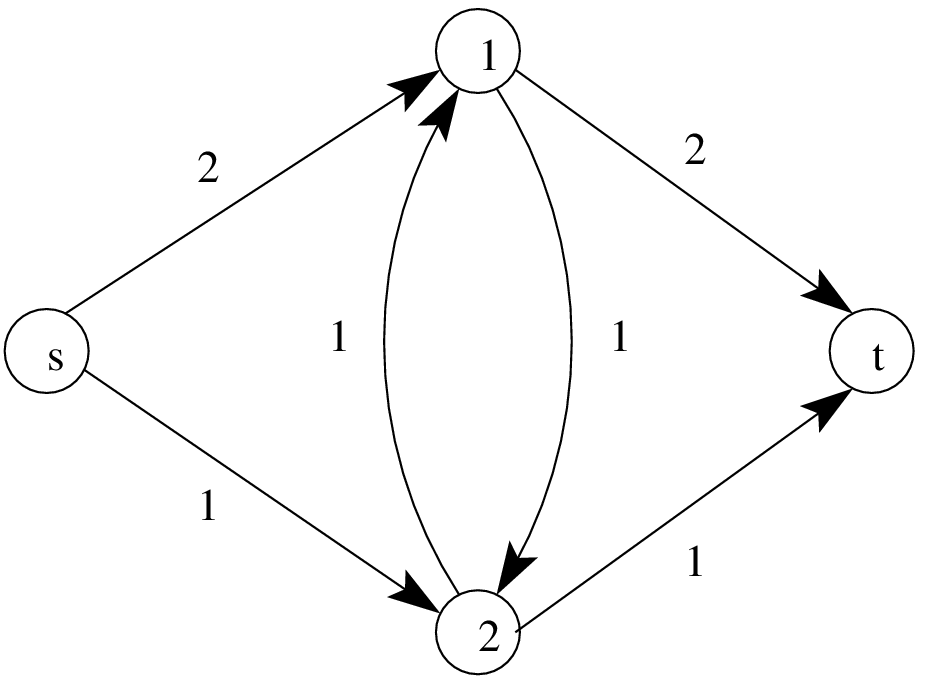
\includegraphics{ex_network.png}
  \caption{An example of a network with $n=4$ vertices and $m=6$ edges. The
  capacities of the edges are shown.}
\label{fig:ex_network}
\end{center}
\end{figure}


In a network flow problem, we assign a {\em flow} to each edge.  There are
two ways of defining a flow: raw (or gross) flow and net flow.

\textbf{Definition}:
\textbf{Raw flow} is a function $r(v,w)$ that satisfies the following properties:   
\begin{itemize}
  \item
    Conservation:  The total flow entering $v$ must equal the total flow leaving 
$v$ for all vertices except $s$ and $t$.\\ 
    \begin{align*}
      \underbrace{\sum_{w\in V} r(w,v)}_{\hbox{incoming flow}}-\underbrace{\sum_{w\in V}r(v,w)}_{\hbox{outgoing flow}}=0, \forall v\in V\setminus \{s,t\}.
    \end{align*}
  \item 
    Capacity constraint: The flow along any edge must be
positive and less than the capacity of that edge.
    \begin{align*}
      0 \le r(v,w)\le u(v,w).
    \end{align*}
\end{itemize}





\begin{figure}[h]
\begin{center}
  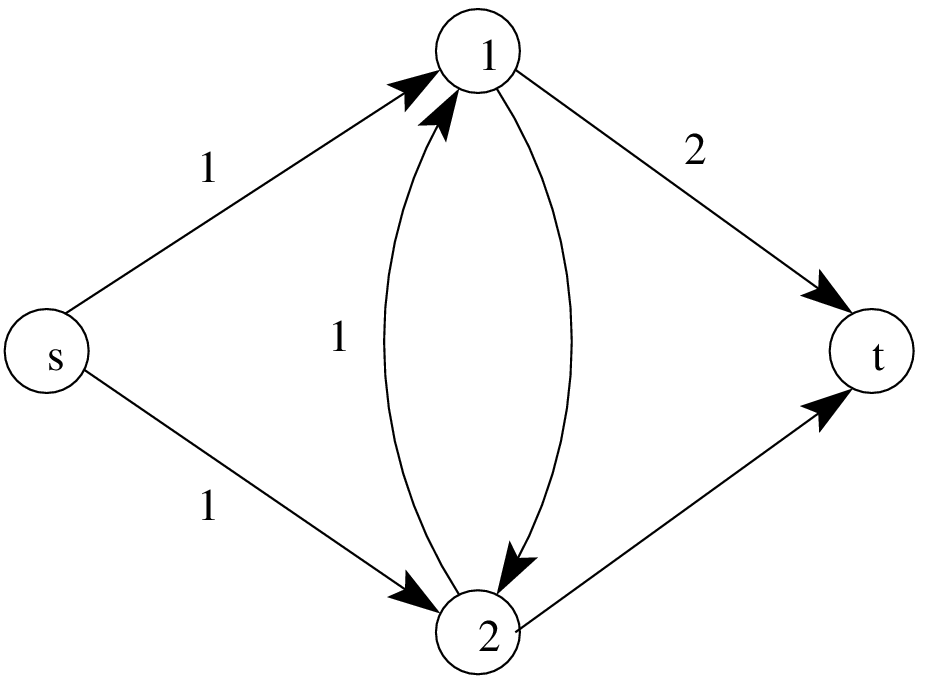
\includegraphics{ex_rawflow.png}
  \caption{An example of a raw flow for the network above. The flow has
  a value of 2.}
\label{fig:ex_rawflow}
\end{center}
\end{figure}


With a raw flow, we can have flows going both from $v$ to $w$ and flow
going from $w$ to $v$.  In a net flow formulation however, we only
keep track of the difference between these two flows.


\textbf{Definition}:
\textbf{Net flow} is a function that satisfies the following conditions:
\begin{itemize}
\item
  Skew symmetry: $f(v,w)=-f(w,v)$.
\item
  Conservation: $\sum_{w\in V} f(v,w)=0$, for all $v\in
  V\setminus\{s,t\}$.
\item
  Capacity constraint: $f(v,w)\le u(v,w)$ for all $v,w\in V$.
\end{itemize}

A raw flow $r(v, w)$ can be converted into a net flow via the formula:
\begin{align*}
  f(v, w) = r(v, w) - r(w, v).
\end{align*}
For example, if we have 7 units 
of flow from $v$ to $w$ and 4 units of flow from $w$ to $v$, then the
net flow from $v$ to $w$ is  $f(v, w) = 3$.  Skew symmetry follows
directly from this formula relating raw flows and net flows.  Because
we can convert from raw flows to net flows, for the rest of the
lecture we consider only net flow problems.

Although skew symmetry relates $f(v, w)$ and $f(w, v)$, it is
important to note that the capacity in one direction $u(v, w)$ is independent of
the capacity in the reverse direction, $u(w, v)$.  

The value of a flow is the sum of the flow on all edges leaving the
source $s$.  We later show that this is equivalent to the sum of all
the flow going into the sink $t$.  The value of a flow represents how
much we can transport from the source to the sink.  Our goal in this
lecture is to solve the maximum flow problem. 

\textbf{Definition}:
The \textbf{value of a flow} $f$ is defined as $|f|=\sum_{v\in V} f(s,v)$.

\textbf{Definition (Maximum flow problem)}: Given a network $G = (V, E)$, find a
feasible flow $f$ with maximum value.





\section{Flow Decomposition and Cuts}

In this section, we show that any feasible flow can be decomposed into
paths from the source to the sink and cycles.  We use this fact to
derive an upper bound on the maximum flow value in terms of cuts of
the network.



\textbf{Lemma} \label{Flow Decomposition}:
We can decompose any feasible flow $f$ on a network $G$ into at
most $m$ cycles and s-t paths. 

\begin{proof}
  The following algorithm extracts the $m$ paths and cycles.
  
  \begin{quote}
    \begin{enumerate}
      \item
        Find a path with positive flow from the node $s$ to node
        $t$. (If the flow is non-zero, there exists at least one such
        path.) 
      \item
        Anti-augment the flow on this path---that is, reduce the flow in
        the path until the flow on some edge becomes 0.
      \item
        Add this path as an element of the flow decomposition.
      \item
        Continue these operations until there are no more paths from
        $s$ to $t$ with positive flow.
      \item
        If there are still some edges with non-zero flow, the
        remaining flow can be decomposed into cycles. Find a cycle in
        the following way: take any edge with non-zero flow and follow
        an outgoing edge with non-zero flow until a cycle is found.
      \item
        Anti-augment on the cycle found.
      \item
        Add the cycle as an element of the flow decomposition.
      \item
        Continue finding cycles until there are no more edges with
        non-zero flow.
    \end{enumerate}
  \end{quote}
  
  Each time we anti-augment a path or a cycle, we zero out the
  flow on some edge. There are at most $m$ anti-augmentations, and,
  consequently, $m$ paths/cycles in the flow decomposition.
\end{proof}


In a network flow problem, it is useful to work with a {\em cut} of the
graph, particularly an {\em s-t cut}.


\textbf{Definition}:
An s-t cut of network $G$ is a partition of the vertices $V$ into 2 groups: $S$ and
$\bar{S}=V\setminus S$ such that $s\in S$ and $t\in \bar{S}$.  

\begin{figure}[h]
\begin{center}
  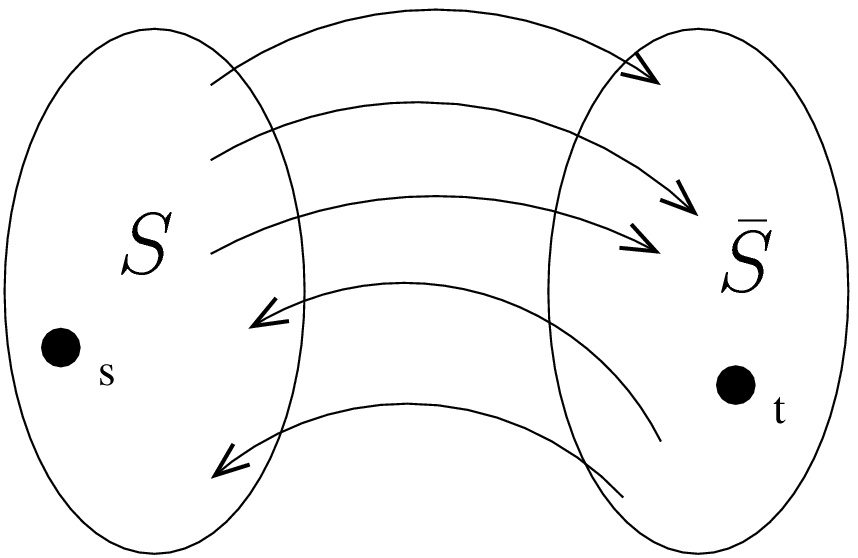
\includegraphics{ex_cut1.png}
  \caption{An illustration of an s-t cut.  There might be both edges from $S$ to $\bar{S}$ and
  from $\bar{S}$ to $S$.}
\label{fig:ex_cut1}
\end{center}
\end{figure}


We will usually represent a cut as the pair $(S, \bar{S})$, or
just $S$.  We generalize the concept of the net flow and the
capacity of an edge to define the net flow and capacity of a cut.


\textbf{Definition}:
The \textbf{net flow} along cut $(S, \bar{S})$ is defined as
\begin{align*}
  f(S)=\sum_{v\in S}\sum_{w\in \bar{S}} f(v,w).
\end{align*}


\textbf{Definition}:
The \textbf{value (or capacity)} of a cut is defined as
\begin{align*}
  u(S)=\sum_{v\in S}\sum_{w\in \bar{S}} u(v,w).
\end{align*}

In summary, the value (or capacity) of a cut is the sum of all values (capacities) of edges that go from $S$ to $\bar{S}$.  Note that direction is important in these definitions.  Capacity along an edge in the reverse direction, from $w \in \bar{S}$ to $v \in S$, does not count. 

\begin{figure}[h]
\begin{center}
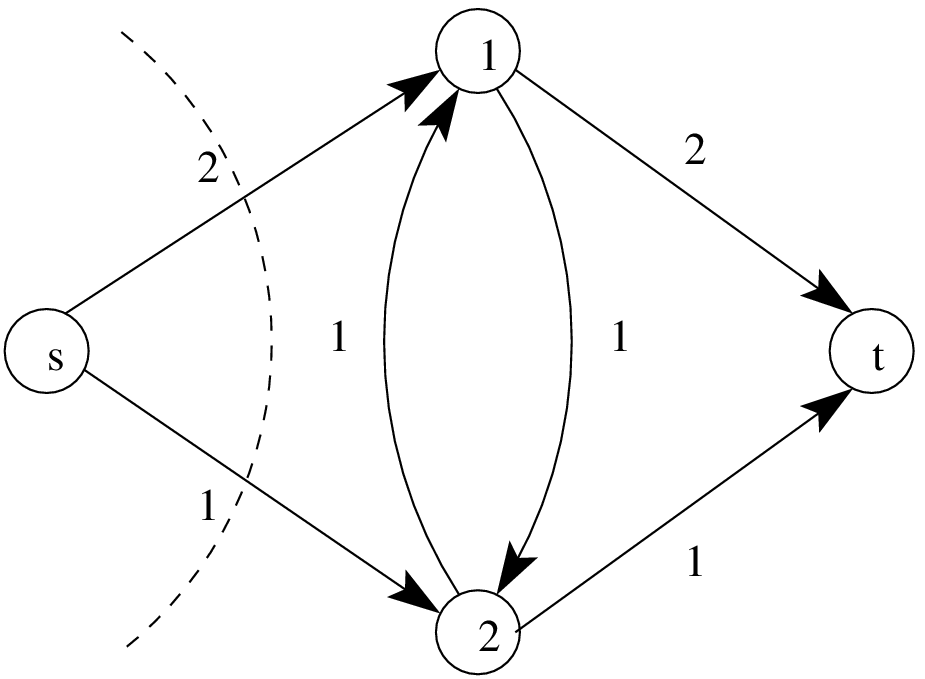
\includegraphics{ex_cut2.png}
\caption{An example of a cut in a network. The s-t cut is represented
  by a dashed line. The value (capacity) of the cut is equal to
  3. This is one of the minimum s-t cuts.}
\label{fig:ex_cut2}
\end{center}
\end{figure}


Working with cuts is useful because of the following lemma:

\textbf{Lemma} \label{All s-t Cuts Same}:
Given a flow $f$, for any cut $S$, $f(S) = |f|$.  In other words,
all s-t cuts  carry the same flow: the value of the flow $f$.

\begin{proof}
We can use Lemma \ref{Flow Decomposition} to prove this statement directly.
We decompose the flow into s-t paths and cycles.  Each s-t path must
end up in $\bar{S}$, so it must go from set $S$ to $\bar{S}$ one more
time than it goes from $\bar{S}$ to $S$.  Therefore, an s-t path
carring $x$ flow along that path contributes exactly $x$ to the value
of the cut.  
A cycle must go from $S$ to $\bar{S}$ the same number of
times as it goes from $\bar{S}$ to $S$, contributing 0 to the value of
the cut.   
Therefore the total value of the cut $S$ is equal to the sum of the
flows along every s-t path, which is equal to $|f|$.  

Alternatively, we can prove the lemma by induction on the size of the
  sets $S$.    For $S={s}$, the claim is true. Now, suppose we move
  one vertex $v$ from $\bar{S}$ to $S$.  The value $f(S)$ changes
  in the following way:
  \begin{itemize}
    \item
      $f(S)$ increases by $f(v,\bar{S})$.
    \item
      $f(S)$ decreases by $f(S,v) = -f(v,S)$.
  \end{itemize}
  In conclusion, the total change in the value of $f(S)$  after moving the
  vertex $v$ from $S$ to $\bar{S}$ is equal to
 $f(v,\bar{S})+f(v,S)=f(v,V)=0$ (by conservation of flow).
\end{proof}


For a flow network, we define a {\em minimum cut} to be a cut of the
graph with minimum capacity.  Then, Lemma \ref{Flow Upper Bound} gives us
an upper bound on the value of any flow.

\textbf{Lemma} \label{Flow Upper Bound}:
If $f$ is a feasible flow, then $|f| \le u(S)$ for any cut $S$. 

\begin{proof}
For all edges $e$, $f(e) \le u(e)$, so $f(S) \le u(S)$ (the flow
across any cut $S$ is not more than the capacity of the cut).  By
Lemma \ref{All s-t Cuts Same}, $|f| = f(S)$, so $|f| \le u(S)$ for any cut
$S$.  
\end{proof}

If we pick $S$ to be a minimum cut, then we get an upper bound on the
maximum flow value.


\section{Max-Flow Min-Cut Theorem}
In this section, we show that the upper bound on the maximum flow
given by Lemma \ref{Flow Upper Bound} is exact.  This is the
max-flow min-cut theorem.

To prove the theorem, we introduce the concepts of a residual network
and an augmenting path.


\textbf{Definition}:
Let $f$ be a feasible flow on a network $G$. The
corresponding \textbf{residual network}, denoted $G_f$, is a network that
has the same vertices as the network $G$, but has edges with
capacities $u_f(v, w) = u(v, w) - f(v, w)$.   Only edges with
non-zero capacity, $u_f(v,w)>0$, are included in $G_f$.

Note that the feasibility conditions imply that $u_f(v,w)\ge 0$ and
$u_f(v,w)\le u(v,w)+u(w,v)$.  This means all capacities in the
residual network will be non-negative.  



\textbf{Definition}:
An \textbf{augmenting path} is a directed path from the node $s$ to node $t$
in the residual network $G_f$.

\begin{figure}[h]
\begin{center}
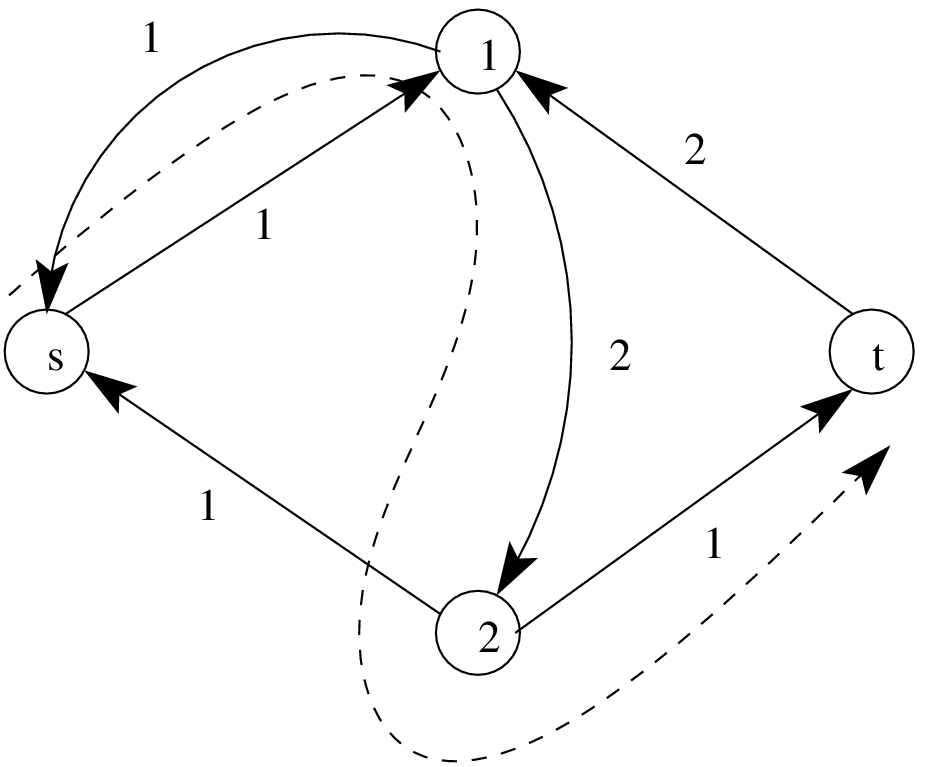
\includegraphics{ex_residual.png}
\caption{An example of a residual network. This residual network
  corresponds to the network depicted in Figure \ref{fig:ex_network}
  and the flow in Figure \ref{fig:ex_rawflow}.  The dashed line
  corresponds to a possible augmenting path.}
\label{fig:ex_residual}
\end{center}
\end{figure}



Note that if we have an augmenting path in $G_f$, then this means we
can push more flow along such a path in the original network $G$.  
To be more precise, if we have an augmenting path $(s, v_1, v_2, \dots v_k,
t)$, the maximum flow we can push along that path is $\min\{u_f(s,
v_1), u_f(v_1, v_2), u_f(v_2, v_3), \dots u_f(v_{k-1}, v_k), u_f(v_{k},
t)\}$.   Therefore, for a given network $G$ and flow $f$, if there exists an
augmenting path in $G_f$, then the flow $f$ is not a maximum flow.  



More generally, if $f'$ is a feasible flow in $G_f$, then $f + f'$ is
a feasible flow in $G$.  The flow $f + f'$ still satisfies
conservation because flow conservation is linear.
The flow $f + f'$ is feasible because we can rearrange the inequality
$f'(e) \le u_f(e) = u(e) - f(e)$ to get $f'(e) + f(e) \le u(e)$.  
Conversely, if $f'$ is a feasible flow in $G$, then the flow $f - f'$ is a
feasible in $G_f$.


Using residual networks and augmenting paths, we can state and prove
the max-flow min-cut theorem.


\textbf{Theorem} (Max-flow min-cut theorem):
In a flow network $G$, the following conditions are equivalent:

\begin{enumerate}
 \item  A flow $f$ is a maximum flow.
 \item  The residual network $G_f$ has no augmenting paths.
 \item  $|f| = u(S)$ for some cut $S$.
\end{enumerate}
These conditions imply that the value of the maximum flow is equal
to the value of the minimum s-t cut: $\max_f |f|=\min_S u(S)$,
where $f$ is a flow and $S$ is a s-t cut.

\begin{proof}
  We show that each condition implies the other two.

\begin{itemize}
\item $1 \Rightarrow 2$:  If there is an augmenting path in $G_f$,
  then we previously argued that we can push additional flow along that path, so
  $f$ was not a maximum flow.  $1 \Rightarrow 2$ is the contrapositive
  of this statement.

\item $2 \Rightarrow 3$:  

If the residual network $G_f$ has no augmenting paths, $s$ and $t$ must be
  disconnected.  Let $S=\{$vertices reachable from $s$ in $G_f \}$. Since $t$ is not
  reachable, the set $S$ describes a s-t cut.


  \begin{figure}[h]
    \begin{center}
      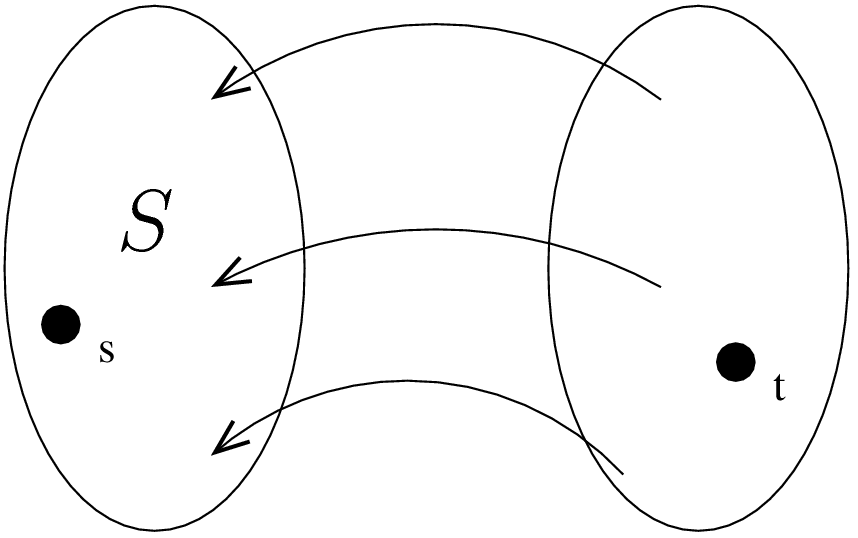
\includegraphics{il_maxmin.png}
      \caption{Network $G_f$ is disconnected. The set $S$ contains all
      the nodes that are reachable from $s$.}
      \label{fig:ex_maxmin}
    \end{center}
  \end{figure}

  By construction, all edges $(v,w)$ crossing the cut have residual
  capacity 0.  This means in the original network $G$, these edges
  have $f(v,w)=u(v,w)$. Therefore, $|f|=f(S)=u(S)$. 

 \item $3 \Rightarrow 1$: 
  If  for some cut $S$, $|f| = u(S)$, we know $f$ must be a maximum
  flow.  Otherwise, we would have a flow $g$ with $|g| > u(S)$, 
  contradicting Lemma \ref{Flow Upper Bound}.

\end{itemize}

From (1) and (3), we know that the maximum flow cannot be less than the value
  of the minimum cut, because for some $S$, $|f| = u(S)$ and $u(S)$ is at least as
  big as the minimum cut value.  Lemma \ref{Flow Upper Bound} tells us
  that the maximum flow can not be greater than the minimum cut
  value.  Therefore, the maximum flow value and the minimum cut value are
  the same.
\end{proof}



\section{Ford-Fulkerson Algorithm}
The Ford-Fulkerson algorithm solves the
problem of finding a maximum flow for a given network. The description
of the algorithm is as follows: 

\begin{quote}
\begin{enumerate}
  \item
    Start with $f(v,w) = 0$.
  \item
    Find an augmenting path from $s$ to $t$ in $G_f$ (using, for example, a depth
    first search or similar algorithms).
  \item
    Use the augmenting path found in the previous step to increase the flow.
  \item
    Repeat until there are no more augmenting paths in $G_f$.
\end{enumerate}
\end{quote}

If the capacities are all integers, then the running time is
$O(m|f|)$.  This is true because finding an augmenting path and
updating the flow takes $O(m)$ time, and every augmenting path we find
must increase the flow by an integer that is at least 1.

In general, if we have integral capacities, then our solution
satisfies an {\em integrality property}: there exists an integral
maximal flow.  This happens because every augmenting path increases
flows by an integer amount.


Since the running time is directly proportional to the value of the
maximal flow, this particular algorithm is only good for cases when
the value $|f|$ is small.  For example, when all capacities are at most
1, the maximum flow $|f|$ is at most $n$.  In general, the algorithm
may be as bad as linear in unary representation of the input.  Figure
\ref{fig:ex_badFF} illustrates a bad case for this form of the
Ford-Fulkerson algorithm.  


We describe such an algorithm as being {\em pseudo-polynomial},
because it is polynomial in terms of variables we care about (but not
necessarily the input).


\begin{figure}[h]
\begin{center}
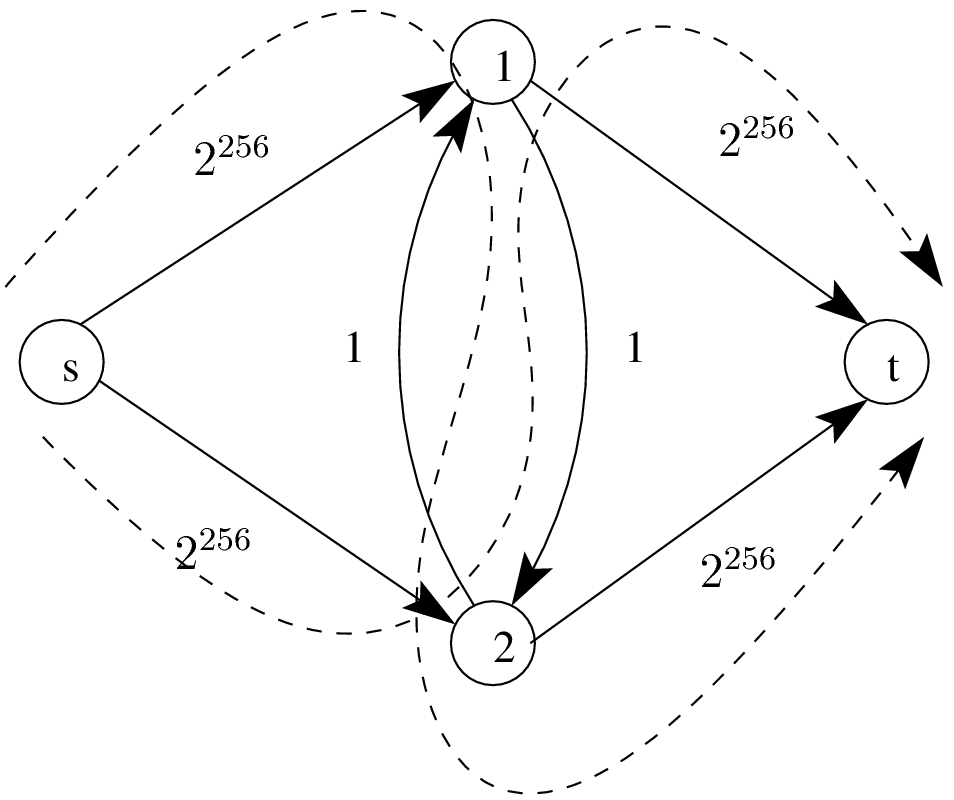
\includegraphics{ex_badFF.png}
\caption{An example for which the Ford-Fulkerson, in the stated form,
  might perform very badly.  The algorithm runs slowly if at each step, the
  augmentation path is either $s\rightarrow 1 \rightarrow 2
  \rightarrow t$ or $s \rightarrow 2 \rightarrow 1 \rightarrow t$ (shown with
  dashed lines). At an augmentation, the flow will increase by at
  most $2$.}
\label{fig:ex_badFF}
\end{center}
\end{figure}


If the capacities are rational, then it can be shown that the
algorithm will finish.  It might, however, require more than $O(m|f|)$
time.  If the capacities are real, the algorithm might never finish,
or even converge to a non-optimal value.  

If we setup better rules for selecting the augmentation paths however,
we might get better results. Before showing some improvements to the
Ford-Fulkerson algorithm, we will introduce some new notions on the
running time of algorithms. 


\textbf{Definition}:
An algorithm is \textbf{psuedo-polynomial} if it is polynomial in the unary
representation of the input.

\textbf{Definition}:
An algorithm is \textbf{weakly polynomial} if it is polynomial in
the binary representation of the input.
    
\textbf{Definition}:
An algorithm is \textbf{strongly polynomial} if it is polynomial in
combinatorial complexity of input. (For example, in the case of
max-flow problem, the algorithm would have to be polynomial in $n$
and $m$.)


\subsection{Improvements to the Ford-Fulkerson Algorithm}

The are at least two possible ideas for improving the Ford-Fulkerson
algorithm. Both of the improvements rely on a better choice of an
augmenting path (rather than a random selection of an augmenting path).

\begin{enumerate}
  \item
    Using breadth-first search, we can choose shortest-length
    augmenting path. With this path-selection rule, the number of
    augmentations is bounded by $n\cdot m$, and thus the running time
    of the algorithm goes down to $O(nm^2)$ time.
  \item
    We can also choose the maximum-capacity augmenting path: the
    augmenting path among all augmenting paths that increases the flow
    the most (max-capacity  augmenting path). It is possible to find
    such a path in $O(m\log n)$ time using a modified Dijkstra's
    algorithm (ignoring the cycles). The number of augmentations will
    be at most $m\ln|f|\le  m\ln(nU)$, where $U=\max\{u(v,w)\}$ (for
    integral capacities). 
\end{enumerate}

In this lecture we prove the time bound for the second
improvement.  
Consider the maximum flow $f$ in the current residual network. We
apply the flow-decomposition lemma, Lemma \ref{Flow Decomposition}
(discarding the cycles because they do not modify $|f|$). There are at most
$m$ paths carrying all the flow, so there must be at
least one path carrying at least $\frac{|f|}{m}$ flow. Therefore, the augmenting
path with maximum capacity increases the flow in the original network
by at least $\frac{|f|}{m}$.   This  decreases the maximum possible flow in
the residual graph  from $|f|$ to $(1-\frac{1}{m})|f|$ (remember, the
smaller is the maximum possible flow in the residual graph, the
greater is the corresponding flow in the original graph). 


We need to decrease the flow $|f|$ by a factor of $(1-\frac{1}{m})$ about
$m\ln|f|$ times before we decrease the max flow in the residual graph
to 1.  This is because

\[|f| \left(1-\frac{1}{m}\right)^{m\ln |f|}\approx
|f|  \left(\frac{1}{e}\right)^{\ln |f|}\approx 1.\]

 In one more step, the residual
graph will have a maximum flow of 0, meaning that the corresponding
flow in the original graph is maximal. Thus, we need $O(m\ln |f|)$
augmentations.  Since one augmentation step takes about $O(m\log
n)$ time, the total running time is $O(m^2 \ln|f| \cdot \ln n)$.  
This algorithm is weakly polynomial, but not strongly polynomial.

\subsection{Scaling Algorithm}

We can also improve the running time of the Ford-Fulkerson algorithm
by using a scaling algorithm.  The idea is to reduce our max flow
problem to the simple case, where all edge capacities are either 0 or 1.

The scaling idea, described by Gabow in 1985 and also by Dinic in
1973, is as follows:

\begin{quote}
\begin{enumerate}
\item
Scale the problem down somehow by rounding off lower order bits.

\item
Solve the rounded problem.

\item
Scale the problem back up, add back the bits we rounded off, and fix
any errors in our solution.
\end{enumerate}
\end{quote}

In the specific case of the maximum flow problem, the algorithm is:

\begin{quote}
\begin{enumerate}
\item
Start with all capacities in the graph at 0.
\item
Shift in the higher-order bit of each capacity.  Each capacity is then
either 0 or 1.
\item
Solve this maximum flow problem.
\item
Repeat this process until we have processed all remaining bits.
\end{enumerate}
\end{quote}

This description of the algorithm tells us how to scale down the
problem.  However, we also need to describe how to scale our algorithm
back up and fix the errors.

To scale back up:

\begin{quote}
\begin{enumerate}
\item
Start with some max flow for the scaled-down problem.  Shift the
bit of each capacity by 1, doubling all the capacities.  If we then
double all our flow values, we still have a maximum flow.
\item
Increment some of the capacities.  This restores the lower order bits
that we truncated.  Find augmenting paths in the residual network to
re-maximize the flow.
\end{enumerate}
\end{quote}


We will need to find at most $m$ augmenting paths.  Before we scaled
our problem back up, we had solved a maximum flow problem, so some cut
in the residual network had 0 capacity.  Doubling all the capacities
and flows keeps this the same.  When we increment the edges however,
we increase the cut capacity by at most $m$: once for each edge.
Each augmenting path we find increases the flow by at least 1, so we
need at most $m$ augmenting paths.

Each augmenting path takes at most $O(m)$ time to find, so we spend
$O(m^2)$ time in each iteration of the scaling algorithm.  If the
capacity of any edge is at most $U$, which is an $O(\lg U)$ bit
number, we require $O(\lg U)$ iterations of the scaling
algorithm.

Therefore the total running time of the algorithm is $O(m^2 \lg U)$.
This algorithm is also a weakly polynomial algorithm.



\end{document}

